\documentclass[11pt,a4paper,oneside]{article}
\usepackage[english]{babel}

\usepackage[T1]{fontenc}
\usepackage[utf8]{inputenc}

\usepackage{geometry} 
\usepackage{color} 
\usepackage{graphicx} 
\usepackage{pifont} 
\usepackage[babel]{csquotes}
\usepackage{textcomp}
\usepackage{upgreek}
\usepackage{amsmath}
\usepackage{textcomp}
\usepackage{amssymb}
\usepackage{latexsym}
\usepackage{pgf}
\usepackage{nicefrac}
\usepackage{enumerate}
\usepackage{stmaryrd}

\usepackage{tgpagella}

\DeclareFontFamily{OT1}{pzc}{}
\DeclareFontShape{OT1}{pzc}{m}{it}{<-> s * [1.10] pzcmi7t}{}
\DeclareMathAlphabet{\mathpzc}{OT1}{pzc}{m}{it}

\newcommand{\ie}{i.\,e.}
\newcommand{\wuppdi}[0]{\hfill\ensuremath{\square}}
\newcommand{\qed}[0]{\vspace{-3mm}\begin{flushright}\textit{q.e.d.}\end{flushright}\vspace{3mm}}
\newcommand{\bred}{\ensuremath{\longrightarrow_\beta}}
\newcommand{\acos}{\textrm{arccos}}
\newcommand{\determ}[1]{\textrm{det}(#1)}
\newcommand{\RR}{\mathbb{R}}
\newcommand{\BB}{\mathbb{B}}
\newcommand{\NN}{\mathbb{N}}
\newcommand{\QQ}{\mathbb{Q}}
\newcommand{\ZZ}{\mathbb{Z}}
\newcommand{\CC}{\mathbb{C}}
\newcommand{\II}{\mathbb{I}}
\newcommand{\kernel}[1]{\textrm{ker}(#1)}
\renewcommand{\epsilon}{\varepsilon}
\renewcommand{\phi}{\varphi}
\renewcommand{\theta}{\vartheta}
\newcommand{\atan}{\mathrm{arctan}}
\newcommand{\rot}{\mathrm{rot}}
\newcommand{\vdiv}{\mathrm{div}}
\newcommand{\shouldbe}{\stackrel{!}{=}}
\newcommand{\sturm}{\texttt{sturm}}
\newcommand{\lemma}{\textbf{lemma}}
\newcommand{\card}{\textrm{card}}
\newcommand{\real}{\textrm{real}}

\newcommand{\isabellehol}{\mbox{Isabelle}\slash HOL}

\geometry{a4paper,left=30mm,right=30mm, top=25mm, bottom=30mm} 

\title{\LARGE User's Guide for the \texttt{sturm} Method\\[4mm]}
\author{\Large Manuel Eberl <eberlm@in.tum.de>\\[1mm]\large Institut für Informatik, Technische Universität München\\[4mm]}

\begin{document}
\begin{center}
\vspace*{20mm}
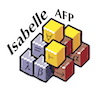
\includegraphics[width=4cm]{isabelle.pdf}
\end{center}
\vspace*{-5mm}
{\let\newpage\relax\maketitle}
\vspace*{10mm}
\tableofcontents
\newpage

\section{Introduction}

The \sturm\ method uses Sturm's theorem to determine the number of distinct real roots of a polynomial (with rational coefficients) within a certain interval. It also provides some preprocessing to decide a number of statements that can be reduced to real roots of polynomials, such as simple polynomial inequalities and logical combinations of polynomial equations.
\vspace*{10mm}

\section{Usage}

\subsection{Examples}
The following examples should give a good overview of what the \sturm\ method can do:
\begin{align*}
&\lemma\ "\card\ \{x::\real.\ (x - 1)^2 * (x + 1) = 0\}\  =\  2"\ \textrm{\textbf{by}\ sturm}\\
&\lemma\ "\mathrm{card}\ \{x::\mathrm{real}.\ -0.010831 < x\ \wedge\ x < 0.010831\ \wedge\\
&\hskip20mm \mathrm{poly}\ [:0, -17/2097152, -49/16777216, 1/6, 1/24, 1/120:]\ \ x\ =\ 0\}\  =\  3"\ \textrm{\textbf{by}\ sturm}\\
&\lemma\ "\card\ \{x::\real.\ x^3 + x = 2*x^2\ \wedge\ x^3-6*x^2+11*x=6\}\  =\  1"\ \textrm{\textbf{by}\ sturm}\\
&\lemma\ "\card\ \{x::\real.\ x^3 + x = 2*x^2\ \vee\ x^3-6*x^2+11*x=6\}\  =\  4"\ \textrm{\textbf{by}\ sturm}\\
&\lemma\ "(x::\real)^2+1 > 0"\ \textrm{\textbf{by}\ sturm}\\
&\lemma\ "(x::\real) > 0\ \Longrightarrow\ x^2+1 > 0"\ \textrm{\textbf{by}\ sturm}\\
&\lemma\ "\llbracket (x::\real) > 0; x \leq 2/3\rrbracket\ \Longrightarrow\ x*x \neq\ x"\ \textrm{\textbf{by}\ sturm}\\
&\lemma\ "(x::\real) > 1\ \Longrightarrow\ x*x > x"\ \textrm{\textbf{by}\ sturm}\\
\end{align*}

\subsection{Determining the number of real roots}
The \enquote{classical} application of Sturm's theorem is to count the number of real roots of a polynomial in a certain interval. The \sturm\ method supports this for any polynomial with rational coefficients and any real interval, \ie $[a;b]$, $(a;b]$, $[a;b)$, and $(a;b)$ where $a\in\QQ\cup\{-\infty\}$ and $b\in\QQ\cup\{\infty\}$.\footnote{The restriction to rational numbers for the coefficients and interval bounds is to the fact that the code generator is used internally, which, of course, does not support computations on irrational real numbers.} The general form of the theorems the method expects is:
$$\card\ \{x::\real.\ a < x \wedge x < b \wedge p\ x = 0\}\ =\ ?n$$
$?n$ should be replaced by the actual number of such roots and $p$ may be any polynomial real function in $x$ with rational coefficients. The bounds $a < x$ and $x < b$ can be omitted for the \enquote{$\infty$} case.\\

Furthermore, the \sturm\ method can instantiate the number $?n$ on the right-hand side automatically if it is left unspecified (as a schematic variable in a schematic lemma). However, due to technical restrictions this also takes twice as long as simply proving that the specified number is correct.

\newpage
\subsection{Inequalities}

A simple special case of root counting is the statement that a polynomial $p\in\RR[X]$ has no roots in a certain interval, which can be written as:
$$\forall x::\real.\ x > a \wedge x < b \longrightarrow p\ x \neq 0$$
The \sturm\ method can be directly applied to statements such as this and prove them.

\subsection{More complex expressions}

By using some simple preprocessing, the \sturm\ method can also decide more complex statements:
$$\card\ \{x::\real.\ x > a\ \wedge\ x < b\ \wedge\ P\ x\}\ =\ n$$
where $P\ x$ is a \enquote{polynomial expression}, which is defined as:
\begin{enumerate}
\item $p\ x= q\ x$, where $p$ and $q$ are polynomial functions, such as $\lambda x.\ a$, $\lambda x.\ x$, $\lambda x.\ x^2$, $\mathrm{poly}\ p$, and so on
\item $P\ x\ \wedge\ Q\ x$ or $P\ x\ \vee\ Q\ x$, where $P\ x$ and $Q\ x$ are polynomial expressions
\end{enumerate}

Of course, by reduction to the case of zero roots, the following kind of statement is also provable by \sturm\ :
$$\forall x::\real.\ x > a\ \wedge\ x < b\ \longrightarrow\ P\ x$$
where $P\ x$ is a \enquote{negated polynomial expression}, which is defined as:
\begin{enumerate}
\item $p\ x\neq q\ x$, where $p$ and $q$ are polynomial functions
\item $P\ x\ \wedge\ Q\ x$ or $P\ x\ \vee\ Q\ x$, where $P\ x$ and $Q\ x$ are negated polynomial expressions
\end{enumerate}

\subsection{Simple ordered inequalities}
For any polynomial $p\in\RR[X]$, the question whether $p(x) > 0$ for all $x\in I$ for a non-empty real interval $I$ can obviously be reduced to the question of whether $p(x) \neq 0$ for all $x\in I$, \ie $p$ has no roots in $I$, and $p(x) > 0$ for some arbitrary fixed $x\in I$, the first of which can be decided using Sturm's theorem and the second by choosing an arbitrary $x\in I$ and evaluating $p(x)$.\\

Using this reduction, the \sturm\ method can also decide single \enquote{less than}/\enquote{greater than} inequalities of the form 
$$\forall x::\real.\ x > a\ \wedge\ x < b\ \longrightarrow\ p\ x < q\ x$$

\subsection{A note on meta logic versus object logic}

While statements like $\forall x::\real.\ x^2+1>0$ were expressed in their HOL notation in this guide, the \sturm\ method can also prove the meta logic equivalents $\bigwedge x::\real.\ x^2+1>0$ and $(x::\real)^2+1>0$ directly.

\section{Troubleshooting}

Should you find that the \sturm\ method fails to prove a statement that it should, according to the above text, be able to prove, please go through the following steps:
\begin{enumerate}
\item ensure that your function is indeed a \emph{real} polynomial. Add an appropriate type annotation if necessary.
\item use a computer algebra system to ensure that the property is indeed correct
\item if this did not help, send the statement in question to \texttt{eberlm@in.tum.de}; it may be a bug in the preprocessing of the proof method.
\end{enumerate}

\end{document}

